\documentclass{article} 
\usepackage{amsmath, amsthm, amssymb, calrsfs, wasysym, verbatim, bbm, color, graphics, geometry, multirow, booktabs}
\usepackage{graphicx}
\usepackage{tikz}
\usepackage{amsmath}
\usepackage{graphicx}
\usepackage{amsmath, amssymb, amsthm}
\usepackage{setspace}
\usepackage{tikz}
\usetikzlibrary{trees, positioning}
\usepackage{pgfplots}
\renewcommand{\baselinestretch}{1.0}
\geometry{tmargin=.75in, bmargin=.75in, lmargin=.75in, rmargin = .75in}  


\newcommand{\R}{\mathbb{R}}
\newcommand{\C}{\mathbb{C}}
\newcommand{\Z}{\mathbb{Z}}
\newcommand{\N}{\mathbb{N}}
\newcommand{\Q}{\mathbb{Q}}
\newcommand{\Cdot}{\boldsymbol{\cdot}}


\title{SP25 8732: Homework 4}
\author{Danbo CHEN}
\date{\today}

\begin{document}

\maketitle
\vspace{.25in}

\section{Question 1}
\textbf{(a) Solution:}
Consider the model 
\[
Y_i = m(X_i, \beta) + \varepsilon_i,
\]
where \( m \) is a function of \( X_i \) and parameters \( \beta \). Define 
\[
g_i = Z_i \varepsilon_i = Z_i \left(Y_i - m(X_i, \beta) \right).
\]
By the assumption that \( \mathbb{E}[Z_i \varepsilon_i] = 0 \), we have 
\[
\mathbb{E}[Z_i (Y_i - m(X_i, \beta))] = 0.
\]

\noindent
Using the sample analog for the population expectation, we get
\[
\bar{g}_n(\beta) = \frac{1}{n} \sum_{i=1}^n g_i(\beta) = \frac{1}{n} \sum_{i=1}^n Z_i \left(Y_i - m(X_i, \beta) \right).
\]

\noindent
Note that \( \bar{g}_n(\beta) \) is an \( L \times 1 \) vector. The GMM estimator minimizes the objective function:
\[
J_n(\beta) = n \times \bar{g}_n(\beta)' W_n \bar{g}_n(\beta),
\]
where \( W_n \) is a positive definite weighting matrix.

\noindent
The first-order condition is given by:
\[
\frac{\partial J_n(\beta)}{\partial \beta} = 2 \times \frac{\partial \bar{g}_n(\beta)'}{\partial \beta} W_n \bar{g}_n(\beta) = 0.
\]

\subsection*{Regularity Conditions}

Under the following regularity conditions, we can derive the asymptotic distribution of \( \hat{\beta}_{GMM} \):
\begin{itemize}[leftmargin=1.5em]
    \item The data \(\{(Y_i, X_i, Z_i)\}_{i=1}^n\) are i.i.d.;
    \item The true parameter \( \beta_0 \) lies inside the parameter space;
    \item \( g_i(\beta) \) is continuously differentiable in a neighborhood \( \mathcal{N} \) of \( \beta_0 \);
    \item \( \hat{W}_n \) is a consistent estimator of \( W \), and \( W \) is positive definite;
    \item \( Q'WQ \) is invertible, where \( Q = \mathbb{E} \left[\frac{\partial g_i(\beta)}{\partial \beta} \right] \);
    \item 
    \[
    \mathbb{E} \left[\sup_{\beta \in \mathcal{N}} \left\| \frac{\partial g_i(\beta)}{\partial \beta} \right\| \right] < \infty;
    \quad \text{and} \quad \Omega = \mathbb{E}[g_i g_i'] \text{ exists and is invertible}.
    \]
\end{itemize}

\noindent
Then, the asymptotic distribution of the GMM estimator is:
\[
\sqrt{n}(\hat{\beta}_{GMM} - \beta) \xrightarrow{d} \mathcal{N}(0, V_\beta),
\]
where 
\[
V_\beta = (Q'WQ)^{-1}(Q'W\Omega WQ)(Q'WQ)^{-1}.
\]

\subsection*{Efficient GMM Estimation}

Efficient GMM estimation is obtained by setting \( W = \Omega^{-1} \). In practice, using the sample analog, we estimate:
\[
\hat{W}_{\text{eff}} = \frac{1}{n} \sum_{i=1}^n \hat{\varepsilon}_i^2 Z_i Z_i',
\]
where \( \hat{\varepsilon}_i \) is not directly observed but estimated from the first-stage GMM as:
\[
\hat{\varepsilon}_i = Y_i - m(X_i, \hat{\beta}^{(1)}),
\]
and \( \hat{\beta}^{(1)} \) is a consistent first-stage estimator of \( \beta \).

\noindent
In the first stage, the weighting matrix can be chosen as the identity matrix or as in two-stage least squares (2SLS).

\subsection*{Remarks}

\begin{itemize}[leftmargin=1.5em]
    \item When \( L = K \) (exact identification), the choice of weighting matrix does not affect the estimator.
    \item When \( L > K \) (over-identification), the choice of an efficient weighting matrix matters for obtaining the most efficient estimator.
\end{itemize}

\section{Question 3}
\textbf{(a) Solution:}

For this exercise, I use the \texttt{JTRAIN} dataset to determine the effect of the job training grant on hours of job training per employee. The basic model for the three years is specified as follows:

\begin{equation}
HRSEMP_{it} = \beta_0 + \delta_1 D88_t + \delta_2 D89_t + \beta_1 GRANT_{it} + \beta_2 GRANT_{i,t-1} + \beta_3 \ln EMPLOY_{it} + C_i + \varepsilon_{it}
\end{equation}

\noindent
To control for unobserved individual effects \(C_i\), I estimate the equation using first differencing:

\begin{equation}
\Delta HRSEMP_{it} = \beta_0 + \delta D89_t + \beta_1 \Delta GRANT_{it} + \beta_2 \Delta GRANT_{i,t-1} + \beta_3 \Delta \ln EMPLOY_{it}
\end{equation}

\begin{center}
    
    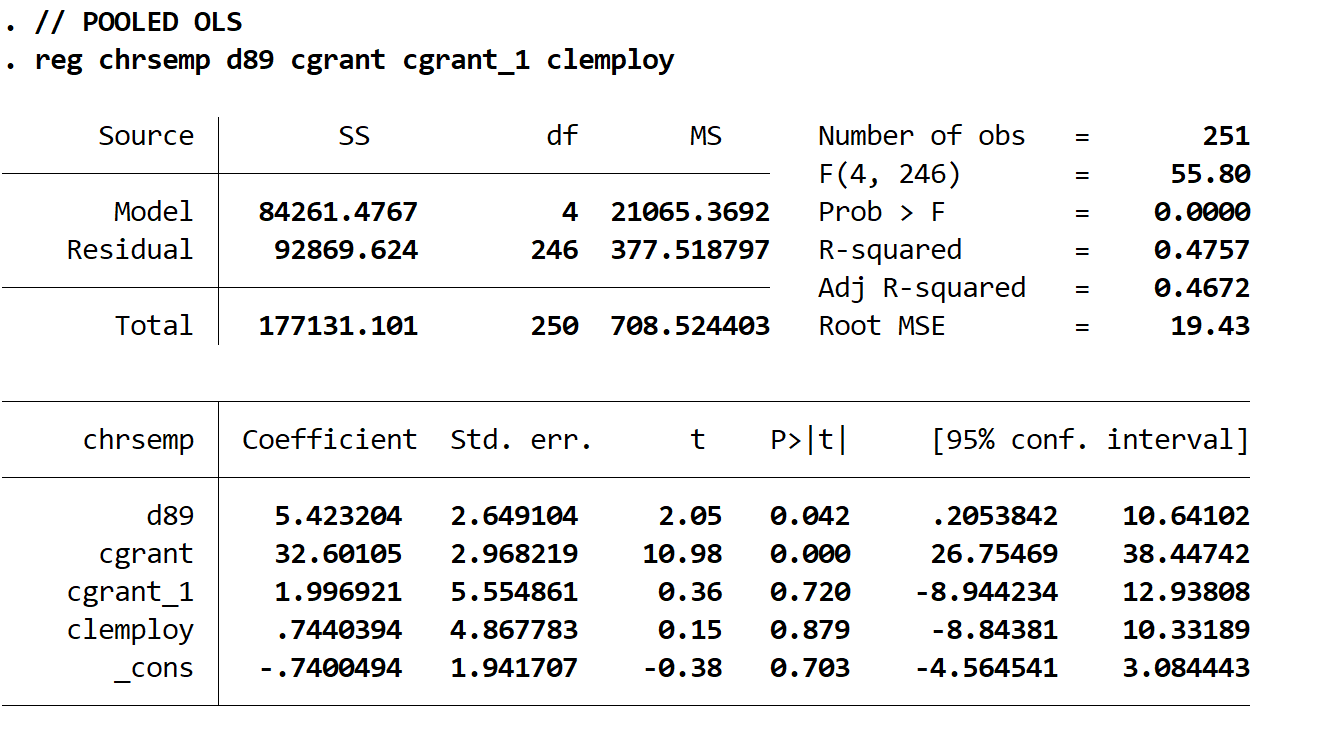
\includegraphics[width=0.8\textwidth]{HW4/P3-1.jpg}
    I use a sample consisting of 251 observations. Among these, 127 observations are included in the regression analysis (\texttt{dup} = 0). Of the remaining 124 observations (251 -- 127), 121 correspond to firms with data for both years, while 3 firms have only one year of data, accounting for the discrepancy between 254 and 251 total potential observations. Additionally, 90 observations are excluded from the regression, which implies that 30 firms in the sample lack data for both years and are therefore not used at all. If complete information were available for all 157 firms in the dataset, we would have a total of 314 observations for estimating the equation.
    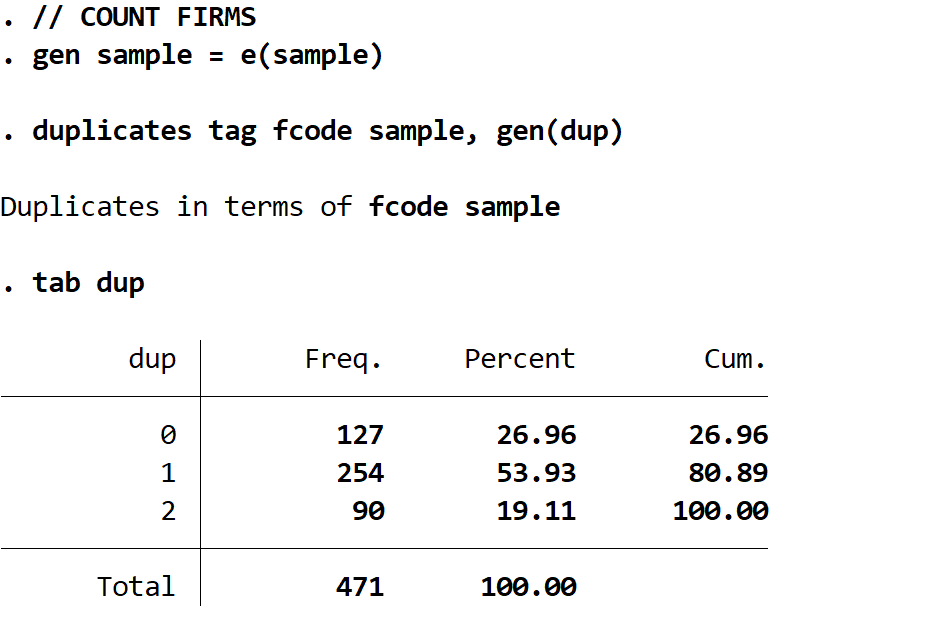
\includegraphics[width=0.8\textwidth]{HW4/P3-2.jpg}

    % 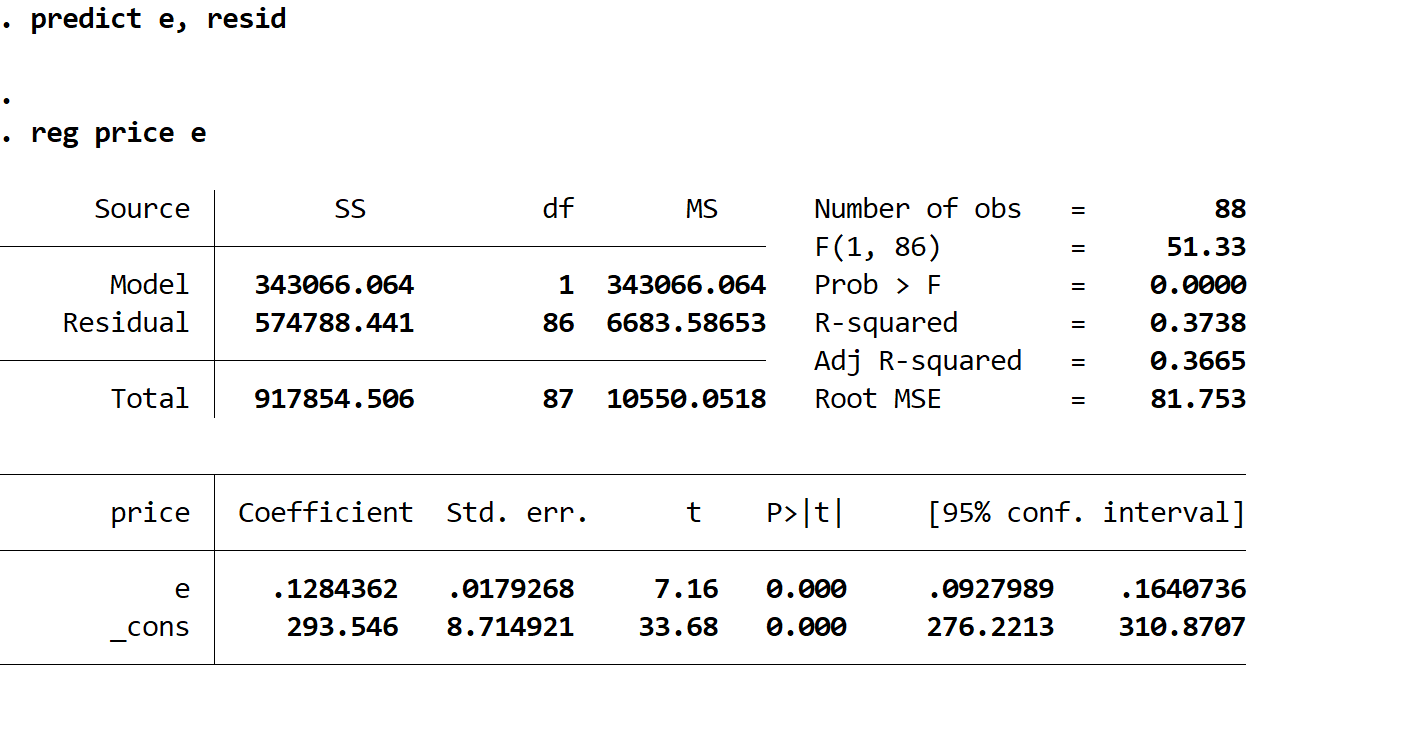
\includegraphics[width=0.8\textwidth]{/P1.C.jpg}

\end{center}

\textbf{(b) Solution:}
The coefficient on the grant variable (\texttt{GRANT}) indicates that firms receiving a grant in the current fiscal year allocate, on average, 32.6 additional hours of training per employee compared to firms that do not receive a grant. This effect is economically substantial and statistically significant, as evidenced by a high \textit{t}-statistic of 10.98.

\textbf{(c) Solution:}
The absence of a significant carryover effect from grants received in the previous year on current-year training expenditures is unsurprising, as grants are generally intended to support training in the year they are awarded. This finding aligns with expectations and suggests that training decisions are not markedly influenced by inertia.

\textbf{(d) Solution:}

The coefficient on the variable representing the number of employees (\texttt{EMPLOY}) indicates a minimal effect: a 10\% increase in employee count leads to only a 0.074-hour increase in training per employee. This effect is notably small and is corroborated by the corresponding low \textit{t}-statistic.

\section{Question 4}
\textbf{(a) Solution:}
Using the \texttt{MURDER} dataset, estimate the model using pooled OLS, disregarding potential unobserved heterogeneity across units. Ensure that the model includes different intercepts for each year.

\begin{center}
    
    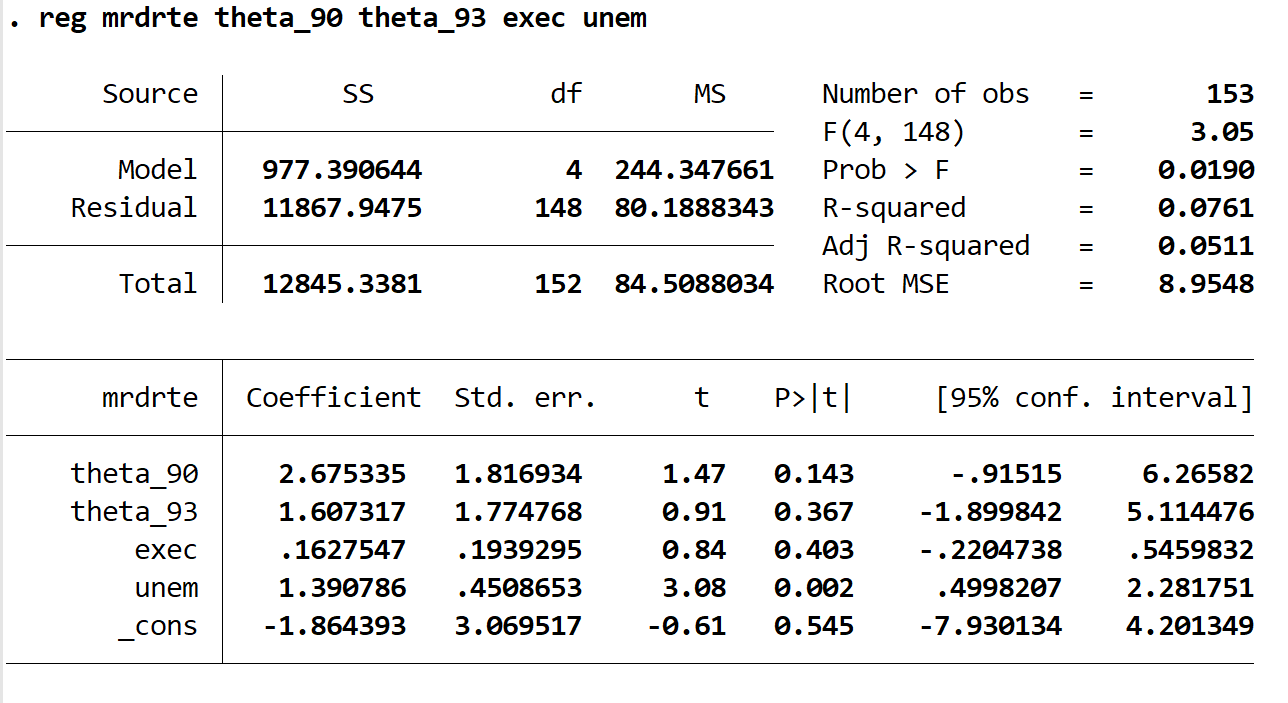
\includegraphics[width=0.8\textwidth]{HW4/P4-1.jpg}
    
\end{center}

\textbf{(b) Solution:}
\begin{center}
    
    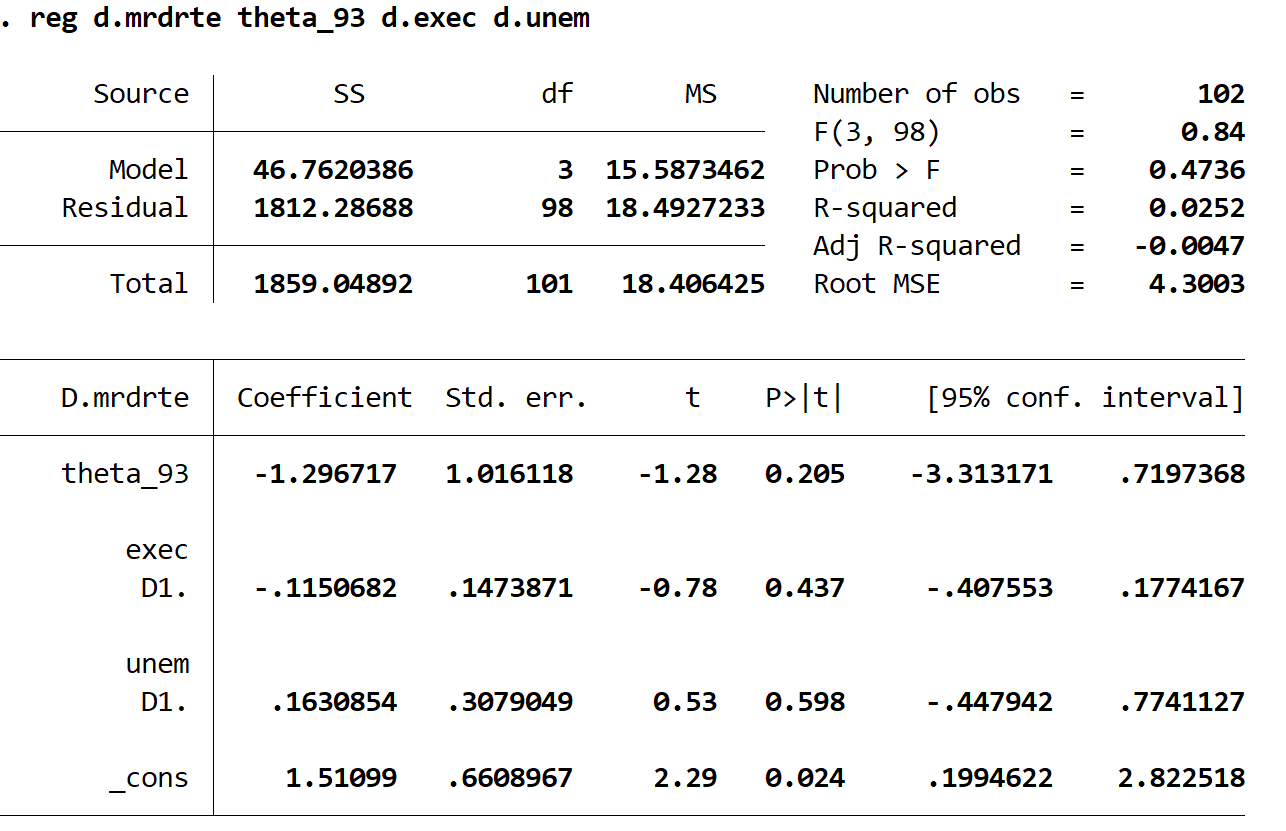
\includegraphics[width=0.8\textwidth]{HW4/P4-2.jpg}
    
\end{center}

\textbf{(c) Solution:}
In the pooled ordinary least squares (OLS) estimation, the coefficient on executions is positive but not statistically significant. In contrast, unemployment exhibits a significant positive effect on the murder rate.

In the first-differenced estimation, the coefficient on executions turns negative; however, it remains statistically insignificant. Additionally, the effect of unemployment becomes less significant under this specification.

\textbf{(d) Solution:}

Considering executions as a variable that could be influenced by previous murder rates poses a potential issue. For instance, if the decision regarding the number of executions is based on prior-year murder rates, a correlation between current-year executions (\(EXEC_{it}\)) and future murder rates (\(\varepsilon_{it}\) and \(EXEC_{it+1}\)) may arise. This would imply a violation of the strict exogeneity assumption. A similar argument applies to unemployment: if current unemployment is correlated with future murder rates, this too would violate the condition of strict exogeneity.

\end{document}





